Um programa de computador é expresso por um conjunto de sentenças em alguma
linguagem de programação.\footnote{Uma sentença (\emph{statement}) pode conter uma ou várias expressões ou instruções.
Uma única instrução numa linguagem de alto nível pode representar múltiplas
instruções de máquinas.
Programas consistem de instruções e expressões.
Uma expressão é um grupo de símbolos que representa um valor.}
A forma como as sentenças de uma linguagem são executadas pelo computador é
definida por um \emph{modelo de computação} \cite{roy2004}.

O código fonte de um programa consiste de uma série de instruções que expressam
uma sequência de comandos a se seguir durante a execução — esse período é
conhecido como \emph{tempo de execução}, do inglês \emph{runtime}.
Tradicionalmente, as sentenças de uma linguagem de programação denotam essa
sequência de forma explícita.
Tais linguagens são baseadas no modelo \emph{imperativo} de computação, e são
denominadas \emph{linguagens imperativas}.

\section{Linguagens de Programação}
\label{sec:org7b5e110}
\label{sec:langs}

Linguagens de programação são mais simples que linguagens naturais, no
entanto, elas ainda podem conter uma sintaxe surpreendentemente rica, um
conjunto de abstrações, e bibliotecas auxiliares.
Esse é essencialmente o caso de linguagens usadas para resolver problemas
reais do dia-a-dia.
\textcite{roy2004} as chamam de linguagens \emph{práticas}, que são “\textelp{}
como a caixa de ferramentas de um mecânico experiente: há várias ferramentas
diferentes para finalidades diferentes e todas estão lá por uma razão.” (p.
33; tradução nossa).

Todas as linguagens de programação possuem elementos primitivos para a
descrição de dados e das transformações, ou processos, aplicados à eles —
como a adição de dois números ou a seleção de um item de uma coleção.
Essas primitivas são definidas por regras de sintaxe — a gramática — e pela
semântica — o significado.

Linguagens imperativas geralmente oferecem comandos para lidar com estado em
tempo de execução, como declaração e atribuição de variáveis, e comandos
para controlar o caminho que o programa deve seguir, como os que decidem a
ordem de execução das sentenças — na literatura essa ordem é chamada de
\emph{fluxo de controle} de um programa.

Durante sua execução o programa segue um caminho de acordo com seu \emph{estado}
interno — ou \emph{memória}, o que um programa se lembra enquanto está ‘rodando’.
Programas com estado interno, ou \emph{statefull} em inglês, são projetados para
lembrar de eventos anteriores ou de interações com o usuário.
A informação recordada é denominada o estado do programa \cite{rouse2005}.

\section{Paradigmas de Programação}
\label{sec:org96c55c0}
Programação é uma disciplina extensa, e linguagens práticas de programação
geralmente são bastante complicadas.
Felizmente, as ideias importantes de linguagens de programação são simples
\cite{roy2009}.
Um \emph{paradigma de programação}:

\begin{citacao}
  \textelp{} é uma abordagem para a programação de um computador baseada em
  uma teoria matemática ou um conjunto coerente de princípios.
  \cite[p.~10; tradução nossa]{roy2009}
\end{citacao}

É mais interessante focar em paradigmas de programação do que em linguagens,
porque há muito menos paradigmas que linguagens, como pode-se notar na Figura
\ref{img:LangsParadigmsConcepts} \cite{roy2009}.
Segundo \textcite{roy2009}:

\begin{citacao}
  Os conceitos são os elementos primitivos básicos usados para construir os
  paradigmas. Muitas vezes dois paradigmas que parecem muitos diferentes (por
  exemplo, programação funcional e programação orientada a objetos) diferem
  por apenas um conceito. (p. 13; tradução nossa)
\end{citacao}

\begin{figure}[ht]
  \caption{Linguagens, paradigmas, e conceitos de programação.} \centering
  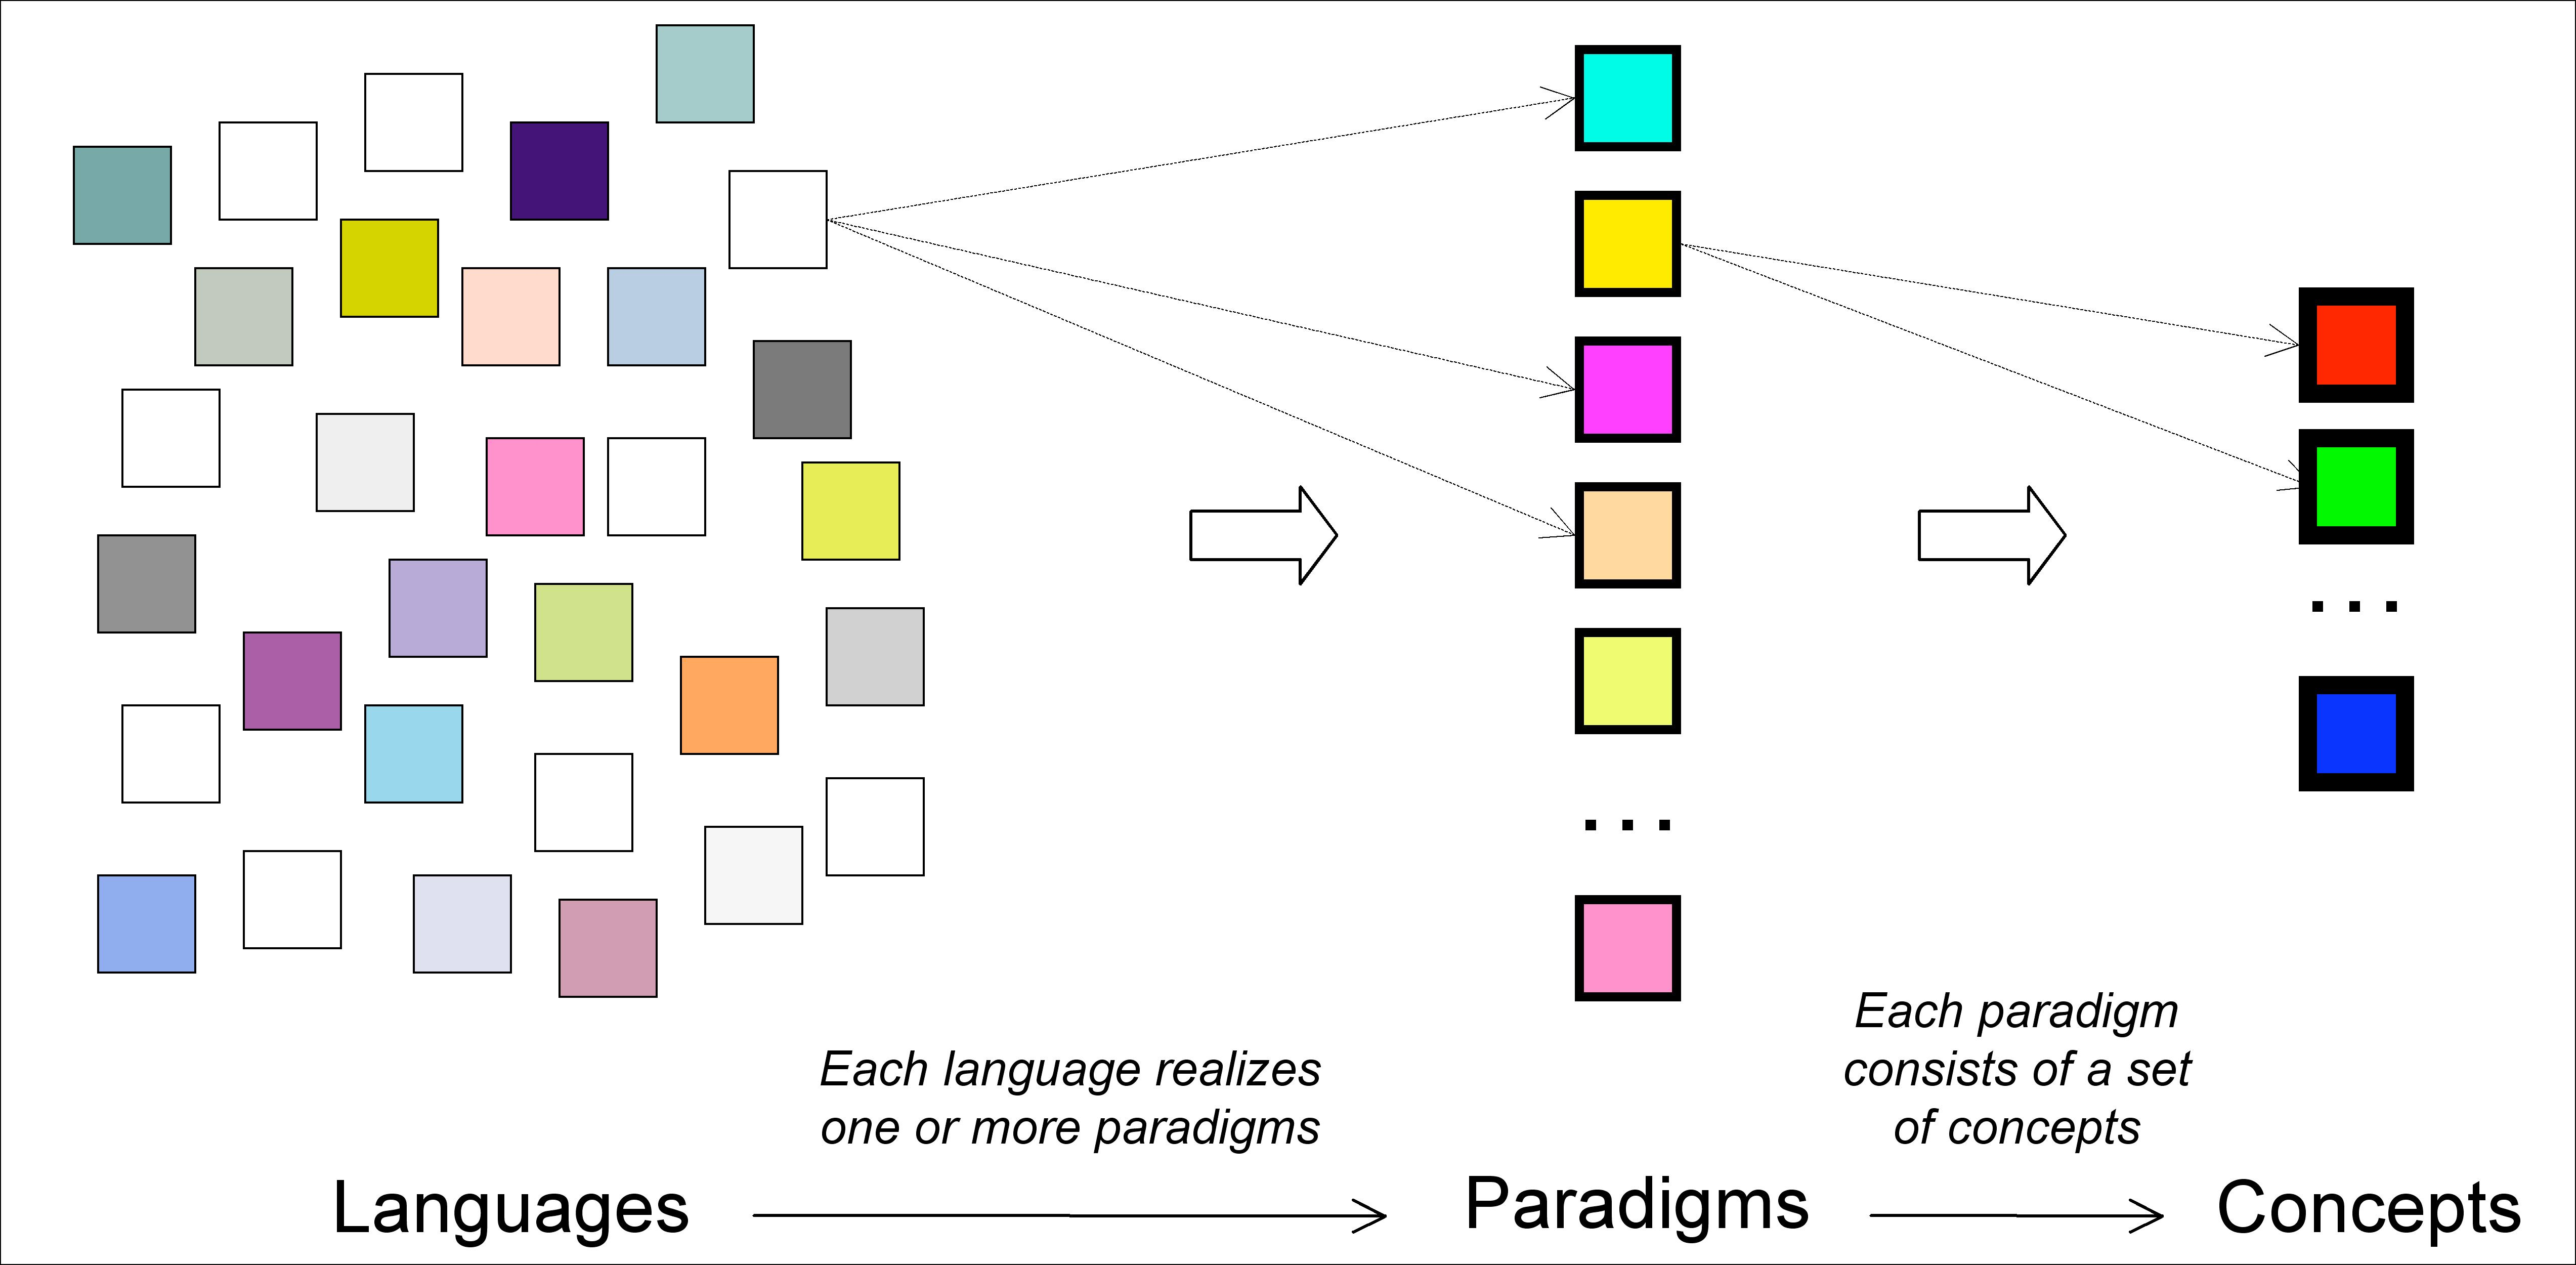
\includegraphics[width=12cm]{./fig/roy2009_languages_paradigms_and_concepts.jpeg}

  \small Fonte: \textcite[p.~12]{roy2009}.
  \label{img:LangsParadigmsConcepts}
\end{figure}

Da mesma forma que em engenharia de software (como um processo) pode-se adotar
diferentes metodologias de desenvolvimento, em linguagens de programação (como
modelos de computação) é desejável utilizar diferentes paradigmas de
programação.
Linguagens tradicionais como Java e C++ dão suporte a um ou dois paradigmas
diferentes.
“Isso é lamentável, pois problemas de programação diferentes precisam de
conceitos diferentes de programação para serem resolvidos claramente.”
\cite[p. 10]{roy2009}.

\textcite{roy2009} defende o uso de um modelo de programação \emph{multiparadigma},
porque:

\begin{citacao}
  Idealmente, uma linguagem deveria dar suporte a vários conceitos de forma
  bem integrada, para que o programador possa escolher os conceitos certos
  sempre que forem necessários, sem que um complique o outro.
  (p.~10; tradução nossa)
\end{citacao}

Apesar de linguagens tradicionais não dar suporte a esse modelo, entender os
conceitos certos pode melhorar a forma de programação, mesmo em linguagens que
não dê suporte direto a eles, assim como programação orientada a objetos é
possível em C com a atitude adequada \cite{roy2009}.

\textcite{roy2009} apresenta quatro modelos importantes que simplificam
programação concorrente em relação à linguagens convencionais: \emph{concorrência
declarativa}, \emph{programação funcional reativa}, \emph{programação síncrona
discreta}, e \emph{programação com restrições}.

No modelo declarativo de concorrência o resultado de um programa pode ser
calculado incrementalmente.
“Se a entrada de um programa concorrente é dada incrementalmente, então o
programa também irá calcular o resultado de saída incrementalmente.”
\cite[p. 238; tradução nossa]{roy2004}.
Esses paradigmas não possuem condições de corrida, \emph{‘race conditions’} em
inglês.
